\chapter{Materiales y Métodos }

\section{Material vegetal.}

Como modelo experimental se utilizaron plantas de \textit{Raphanus sativus} (r\'abano). Las plantas se mantuvieron expuestas a la luz solar de forma indirecta, por un tiempo de aproximadamente $15$ días, manteniéndose  en condiciones constantes de luminosidad y de disponibilidad de agua y nutrientes. 

\section{Diseños experimentales.}

Se describen dos dise\~nos experimentales que permiten la evaluaci\'on de la actividad de las enzimas de defensa en plantas de \textit{R. sativus} sometidas y no sometidas a estr\'es salino. 

\subsection{Primer dise\~no experimental: Actividad enzim\'atica en plantas no sometidas a estr\'es salino.} \label{d1}

Para este experimento se utilizó un total de 15 plantas de r\'abano, divididas en 5 grupos experimentales (3 plantas por grupo): Control negativo (planta sin tratar), Etanol (EtOH) (0,01 mg/mL), DI-31 (0,01 mg/mL), MH-5 (0,01 mg/mL) y Ácido Salicílico (AS) (0,01 mg/mL) como control positivo del experimento (Fig. \ref{plantas}). \\

Para su cultivo se prepar\'o una mezcla de tierra/humus en partes iguales en un semillero germinador y se sembraron dos semillas en cada división. Cada grupo experimental fue sometido a un único tratamiento, los cuales fueron aplicados por aspersión foliar (con el uso de un nebulizador) en tres dosis: a las 0, 24 y 48 horas luego de comenzado el experimento.\\

Las hojas de las plantas se recolectaron a las 24, 48 y 72 horas después de haber comenzado el ensayo. Las muestras fueron maceradas en nitrógeno líquido y almacenadas a $-20^oC$ hasta su procesamiento. \\

%\begin{table}[h]
%	\caption{Esquema de trabajo para cada uno de los tiempos. El primer n\'umero asignado a cada planta representa el tiempo de recogida de la muestra y el segundo representa el tratamiento.}
%	\label{esquema1}
%	\begin{center}
%		\begin{tabular}{|c|M{25mm}|M{25mm}|M{25mm}|M{25mm}|M{25mm}|c|}
%			\hline 
%			\textbf{} & \textbf{Nada} & \textbf{EtOH} & \textbf{DI-31} & \textbf{MH-5} & \textbf{AS} \\ 
%			\hline 
%			$24 \; horas$ &  $Planta \; 1.1$ & $Planta\; 1.2$  & $Planta\; 1.3$ & $Planta\; 1.4$ & $Planta\; 1.5$ \\ 
%			\hline 
%			$48 \; horas$ &  $Planta\; 2.1$ & $Planta \;2.2$  & $Planta \;2.3$ & $Planta \;2.4$ & $Planta\; 2.5$ \\ 
%			\hline 
%			$72 \; horas$ &  $Planta \;3.1$ & $Planta \;3.2$  & $Planta \;3.3$ & $Planta \;3.4$ & $Planta \;3.5$ \\
%			\hline 
%		\end{tabular} 
%	\end{center}
%\end{table}
%
%\normalsize


\begin{figure}[hbtp]
	\centering
	\includegraphics[scale=0.70]{Imagenes/plantas}
	\caption{Primer dise\~no experimental: Plantas de \textit{Raphanus sativus} no sometidas a estr\'es salino. Tratamientos: AS, DI-31, EtOH y control negativo.}
	\label{plantas}
\end{figure}

\subsection{Segundo dise\~no experimental: Actividad enzim\'atica en plantas sometidas a estr\'es salino (NaCl).} \label{d2{}}

Este dise\~no se basa en la metodolog\'ia propuesta por \cite{muthukumarasamy2000enhancement} (con modificaciones) y permite estudiar el efecto de los compuestos DI-31 y MH-5 en la actividad de las diferentes enzimas ante estr\'es por salinidad. El dise\~no de los tratamientos se muestra en la tabla \ref{Ttos}. \\

\begin{table}[h]
	\caption{Dise\~{n}o de los tratamientos.}
	\label{Ttos}
	\begin{center}
		\begin{tabular}{|c|l|}
			\hline 
			\textbf{ } & \textbf{Tratamientos} \\ 
			\hline 
			1 & semillas con $H_2O$ destilada \\ 
			\hline 
			2 & NaCl  \\ 
			\hline 
			3 & NaCl + DI-31 ($1 \; mg/mL$) \\ 
			\hline 
			4 & NaCl + MH-5 ($1 \; mg/mL$) \\ 
			\hline 
			5 & NaCl + AS ($1 \; mg/mL$) \\ 
			\hline 
		\end{tabular} 
	\end{center}
\end{table}

\begin{figure}[hbtp]
	\centering
	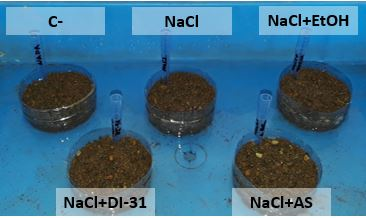
\includegraphics[scale=0.8]{Imagenes/plantas2}
	\caption{Segundo dise\~no experimental: Semillas de \textit{Raphanus sativus} previas a su germinaci\'on sometidas a estr\'es salino. Tratamientos: control negativo, NaCl, NaCl+EtOH, NaCl+DI-31 y NaCl+AS.}
	\label{plantas2}
\end{figure}

Para crear las condiciones de estr\'es salino se utiliz\'o una soluci\'on de NaCl $80\;mM$, ya que esta concentraci\'on disminuye la masa seca en un $50\%$ respecto al control \citep{muthukumarasamy2000enhancement}.\\

Previo a la siembra, se incubaron las semillas de r\'abano por tres horas en una soluci\'on que conten\'ia cada uno de los tratamientos utilizados, lo que constituye una de las diferencias fundamentales entre los dise\~nos experimentales propuestos. Est\'a ampliamente informado en la literatura que las incubaciones previas en agua o soluciones de varias sustancias afectan positivamente los rasgos tanto de la semilla, como del reto\~no \citep{burgass1984evidence, bradford1986manipulation, taylor1998seed, mcdonald2000seed}.\\

Posteriormente se sembraron diez semillas en cada recipiente relleno de una mezcla de tierra/humus en partes iguales. Los grupos experimentales fueron irrigados con las soluciones descritas anteriormente cada 5 días, durante un período de 30 días. Se recolectaron las hojas de las plantas a los 15 y 30 días después de la primera irrigación y se almacenaron a $-20^oC$ hasta su posterior procesamiento.

%\begin{table}[h]
%	\caption{Cronograma del experimento.}
%	\label{cron}
%	\begin{center}
%		\begin{tabular}{|c|l|}
%			\hline 
%			D\'ia 1 & Sembrado. Primera aplicaci\'on de los tratamientos. \\ 
%			\hline 
%			D\'ia 5 & Segunda aplicaci\'on de los tratamientos.  \\ 
%			\hline 
%			D\'ia 10 & Tercera aplicaci\'on de los tratamientos. \\ 
%			\hline 
%			D\'ia 15 & Recogida del primer grupo experimental.  Cuarta aplicaci\'on de los tratamientos  \\ 
%			\hline 
%			D\'ia 20 & Quinta aplicaci\'on de los tratamientos. \\ 
%			\hline 
%			D\'ia 25 & Sexta aplicaci\'on de los tratamientos. \\ 
%			\hline 
%			D\'ia 30 & Recogida del segundo grupo experimental. \\ 
%			\hline 
%		\end{tabular} 
%	\end{center}
%\end{table}
%
%\normalsize

\section{Metodolog\'ias para la extracci\'on de enzimas.}

Para la preparación de los extractos enzimáticos crudos se utilizaron dos protocolos diferentes. 

\subsection{Protocolo de extracci\'on propuesto por \cite{liu2010exogenous}, con modificaciones.} \label{p1}

Se maceraron $500 \; mg$ de tejido vegetal, utilizando un mortero de cerámica, en nitrógeno líquido, para mantener baja la temperatura y asegurar la ruptura tisular. A la muestra pulverizada se le añadió $1\;mL$ de la Solución de Extracción (Fosfato de Sodio $50\;mM$, EDTA dis\'odico $1\;mM$, $2\%$ Polivinil Pirrolidona (PVPP), pH 7.0; $4^oC$).\\

Las muestras fueron centrifugadas a $10\;000\;g$ por $5$ minutos. El sobrenadante fue transferido a tubos limpios y utilizado para la cuantificación de proteínas y los ensayos enzimáticos de SOD, CAT y PPO. \\

\subsection{Protocolo de extracci\'on propuesto por \cite{baquero2005catalase}, con modificaciones.} \label{p2}

En un mortero de cer\'amica se maceraron $500\;mg$ de material vegetal en nitr\'ogeno l\'iquido, para asegurar la baja temperatura y la ruptura tisular. \\

Una vez triturado el tejido, se a\~nadi\'o al mortero $1\;mL$ de Acetona pura para an\'alisis y se macer\'o nuevamente. El macerado se transfiri\'o a un tubo de microcentr\'ifuga, se incub\'o a $4^oC$ durante 30 minutos para obtener un precipitado proteico y se desech\'o el sobrenadante de acetona utilizando una micropipeta. Este proceso se realiz\'o nuevamente y el sobrenadante se elimin\'o mediante evaporaci\'on al vac\'io con un \textquotedblleft SpeedVac \textquotedblright. \\

El precipitado final se resuspendi\'o con $1\;mL$ de una soluci\'on tamp\'on de Fosfato de Potasio ($200\;mM$, pH 6.8) y se mantuvo bajo agitación continua por $24$ horas a $4^oC$. Posteriormente, las muestras se centrifugaron a 10 000 g durante 20 minutos y se desech\'o el precipitado. El sobrenadante fue utilizado para la cuantificación de proteínas y los ensayos enzimáticos de SOD y PPO.\\

\section{Determinaci\'on de la concentración de proteínas mediante el m\'etodo Bradford.}

La concentraci\'on de prote\'inas se determin\'o siguiendo la metodolog\'ia propuesta por \cite{bradford1976rapid}, con modificaciones. Se emple\'o el Reactivo de Bradford, el cual contiene como colorante Azul Coomassie Brillante G-250 (CBBG, por sus siglas en inglés). La Alb\'umina de Suero Bobino (BSA, según sus siglas en inglés) se emple\'o como prote\'ina est\'andar.  

\subsection {Medición de la proteína estándar.}

Partiendo de una soluci\'on $1\;mg/mL$ de BSA se prepararon diluciones seriadas, de manera que cada muestra analizada contaba con: $100\;\mu g$; $50\;\mu g$; $25\;\mu g$; $12.5\;\mu g$; $6.25\;\mu g$ y $3.125\;\mu g$. De cada diluci\'on fueron a\~nadidos $100 \;\mu L$ en tubos de ensayo diferentes y se adicion\'o el Reactivo de Bradford necesario para un volumen final de $3 \; mL$. Las muestras se incubaron durante 20 minutos a temperatura ambiente. La DO de cada muestra se midi\'o a $595 \;nm$ en un espectrofotómetro de luz visible (UV-1800 UV/Visible, China) \citep{kruger2009bradford}.

\subsection {Cuantificación de proteínas en el extracto enzim\'atico.}

Este proceso se realiz\'o de forma similar a la descrita anteriormente, utilizando un volumen del extracto enzim\'atico de concentraci\'on proteica desconocida, contenido en el intervalo analizado en la prote\'ina est\'andar. 

\section{Ensayos enzimáticos.} 

Se describen los protocolos utilizados para la medici\'on de la actividad de las enzimas SOD, CAT y PPO.

\subsection{Super\'oxido Dismutasa (SOD).}

La cuantificaci\'on de la actividad enzim\'atica de SOD se realiz\'o mediante el m\'etodo colorim\'etrico propuesto por \cite{ma2009spectroscopic}, con modificaciones.\\ 

Este m\'etodo se basa en la estimaci\'on de la inhibici\'on que produce la actividad de la enzima SOD en la autoxidaci\'on del Pyrogallol (\'acido 1,2,3-trihidroxibenzoico). El $50\%$ de la inhibici\'on es equivalente a una unidad de SOD  \citep{pandey2014oxidative}. \\

En una cubeta de vidrio se a\~nadieron $2\;700\;\mu L$ de soluci\'on tamp\'on Tris-HCl $50\;mM$ EDTA dis\'odico $1\;mM$ (pH 8.2), $100\;{\mu}L$ de extracto enzim\'atico y $200\;{\mu}L$ de Pyrogallol a diferentes concentraciones (10 mM; 6,4 mM; 3,2 mM; 1,6 mM y 0,8 mM), para un volumen final de $3\;000{\mu}L$ (3 mL). \\

La soluci\'on de Pyrogallol se prepar\'o a $15\;mM$ en $1\;M$ de HCl, solución que es posible almacenar hasta 3 meses \citep{masayasu1979simplified}. En el momento del ensayo, se diluyó a las concentraciones mencionadas anteriormente. \\

El blanco del experimento se prepar\'o a\~nadiendo todos los componentes del ensayo, excepto el extracto (que fue sustituido por $H_2O$ destilada) a fin de determinar la velocidad basal de autoxidación del Pyrogallol en la soluci\'on. Este proceso de inhibici\'on de la autoxidaci\'on del Pyrogallol se monitore\'o a partir de la medici\'on de la DO a $240\;nm$, cada 15 segundos, durante 3 minutos, a $25^oC$, en un espectrofotómetro de luz visible (UV-1800 UV/Visible, China). \\

%Auto-oxidation of pyrogallol was monitored by recording the kinetics of the reaction mixture containing 2.94 ml of Tris-HCl buffer (50 mM, pH 8.2) 1 mM DETAPAC (Sigma) and 60 µl pyrogallol (20 mM prepared in 10 mM HCl ), on a UV-VIS spectrophotometer (ATI - Unicam, UK) at 420 nm. For SOD assay, 0.2 ml enzyme extract was added to 2.74 ml of the Tris-HCl buffer and the absorbance was adjusted to zero. The reaction was initiated by adding 60 µl of pyrogallol and the change in absorbance was recorded at 420 nm.

Para el c\'alculo de la actividad de SOD, se utilizaron los valores de DO obtenidos tanto para el blanco, como para la muestra. Para ello se siguieron las siguientes ecuaciones, en el orden referido \citep{pandey2014oxidative}:

\begin{equation}
Tasa \; de \; autoxidaci\acute{o}n \; del \; Pyrogallol =\frac {[DO(420) \; final \; - \; DO(420) \; inicial]} {[Tiempo \; de \; ensayo \; (min)]}
\label{tasapyr}
\end{equation}

\begin{equation}
Tasa \; de \; SOD =\frac {[DO(420) \; final \; - \; DO(420) \; inicial]} {[Tiempo \; de \; ensayo \; (min)]}
\label{tasasod}
\end{equation}

\begin{equation}
Inhibici\acute{o}n \; (I) ={Tasa \; de \; autoxidaci\acute{o}n \; del \; Pyrogallol} - {Tasa \; de \; SOD}
\label{inh}
\end{equation}

\begin{equation}
Inhibici\acute{o}n = {\frac{Inhibici\acute{o}n \; (I)} {Tasa \; de \; autoxidaci\acute{o}n \; del \; Pyrogallol} * 100}
\label{inhporc}
\end{equation}

\begin{equation}
50\% \; de \; Inhibici\acute{o}n ={1 \; unidad \; de \; SOD} \rightarrow \% \; Inhibici\acute{o}n \;  \; de \;  X  = \frac{X}{50} \; unidades \; de \; SOD
\label{50inh}
\end{equation}

\begin{equation}
Factor \; de \; diluci\acute{o}n \; 1 = \frac{V (de \; la \; mezcla \; de \; ensayo)}{V (del \; extracto \; enzim\acute{a}tico \; en \; la\; mezcla \; de \; ensayo)}
\label{fd1}
\end{equation}

\begin{equation}
Factor \; de \; diluci\acute{o}n \; 2 = \frac{V (total \; del \; extracto \; enzim\acute{a}tico)}{V (del \; extracto \; enzim\acute{a}tico \; utilizado \; en\; el \; ensayo)}
\label{fd2}
\end{equation}

\begin{equation}
Factor \; de \; diluci\acute{o}n \; total \; (FD) ={Factor \; de \; diluci\acute{o}n \; 1 \; * \; Factor \; de \; diluci\acute{o}n \; 2}
\label{FD}
\end{equation}

\begin{equation}
Actividad \; de \; SOD \; (unidades \; mg^{-1} \; MF) = \frac{unidades \; de \; SOD \; * \; FD}{MF \; de \; la \; muestra} 
\label{act}
\end{equation}

\medskip
\medskip

El Factor de Diluci\'on 2 (Ecuaci\'on \ref{fd2}) no se utiliz\'o en este ensayo, pero es importante para el c\'alculo de la actividad enzim\'atica total de una planta o de un \'organo completo de la misma.

\subsection{Catalasa (CAT).}

Para la cuantificación de la actividad CAT, se sigui\'o la metodolog\'ia propuesta por \citep{chance1955136}, con modificaciones. \\

El extracto enzim\'atico utilizado fue el obtenido mediante el protocolo de extracci\'on propuesto por \cite{liu2010exogenous}, con modificaciones. En una cubeta de cuarzo se a\~nadieron $1\;500\;{\mu}L$ de soluci\'on tamp\'on Fosfato de Potasio $50\;mM$ (pH 7.0), $500\;{\mu}L$ de $H_2O_2$ a dos concentraciones diferentes ($5\;mM$ y $50\;mM$) y $100\;{\mu}L$ de extracto enzimático, para un volumen final de $3\;000\;{\mu}L$ ($3\;mL$). Se utiliz\'o como blanco los mismos componentes referidos anteriormente, con excepción del extracto enzimático (que fue sustituido por $H_2O$ destilada). \\

El $H_2O_2$ $30\%$ se diluy\'o en soluci\'on de Fosfato de Potasio $50\;mM$, en el momento del ensayo. Se ajust\'o la DO de esta solución a $2,05\;cm^{-1}$. Se monitore\'o la disminución de  $H_2O_2$ a partir del decremento de absorbancia, utilizando un espectrofotómetro de luz ultravioleta (\textit{Thermo Scientific spectronic Genesys 10UV}, Estados Unidos) a $240\;nm$ a intervalos de 15 segundos, durante 5 minutos, a $25^oC$. \\

Para calcular la actividad enzimática espec\'ifica se utiliz\'o el coeficiente de extinción del  $H_2O_2$ $39.4\;mM^{-1}cm^{-1}$ y se expresa en $nmol$ de $H_2O_2$ por miligramo de masa fresca (MF) por minuto $(nmol (H_2O_2)mg^{-1}MF^{-1}min^{-1})$.

%ACTIVIDAD CATALASA

%Mezcla de reacción (en cubeta de cuarzo)
%.
%Blanco	Muestra
%Buffer fosfato 50 mM pH 7	1.6 mL	1.5 mL
%%H2O2  50 mM	500 L	500  L
%%Extracto enzimático	--	100  L
%
%%Añada 1,5 mL de solución amortiguadora a la cubeta, 500 µL de H2O2 50mM  y 100 μL de muestra, tape y homogenice por inversión. Lea a los 10 y 70 seg. a 240nm.
%%Siga el procedimiento anterior para determinar la diferencia de densidad óptica que se produce al  reemplazar los 100 L de muestra por solución amortiguadora de fosfato (blanco). Antes de leer el  blanco ajustar a cero absorbancia con solución amortiguadora de fosfato.
%Nota: En presenciasdeactividad Enzimática se observa unadisminuciónela densidad  ópticadelmedio
%NotA: SI CON ESTAS CANTIDADES NO DA BIEN PROBAR  CON LA METODOLOGIA Y CONCENTRACIONES DADAS POR BIOCHEMICA INFORMATION
%
%Cálculos
%Calcule inicialmente:
%%ΔDOmuestra= DO70seg_DO10seg
%%ΔDOblanco= DO70seg_DO10seg
%%Se utilizara el coeficiente de extinción 40 mM-1 cm-1 para el  H2O2 a una λ=240nm 
%%CmM = DO/ ε b
%%donde ε esel chef deextinción y b es el paso deluz de la cubeta: 1cm
%%[(ΔDOmuestra_ ΔDOblanco)] / (40 mM-1 cm-1. cm) = concentración (mmol) de H2O2 descompuesta en un tiempo de 60 segundos (1 minuto) por cada litro de solución.
%%Si tenemos en cuenta del volumen total de la cubeta en la misma se descompuso una cantidad de peroxido igual a:
%
%%[(ΔDOmuestra_ ΔDOblanco)] = A
%
%[A/40] . 2.1/1000 = milimoles de peroxido descompuesto en la cubeta. Esta descomposición fue provocada por 100 microlitors del extracto enzimático.
%Ahora hay que conocer que cantidad de proteína hay en ese volumen d3e extracto enzimatico para expresar la actividad en función de la proteína.
%
%Referencias
%1- Boehringer Mannheim. Biochemical Information. A revised biochemical reference source. Enzymes for routine (1st edition), Germany: Boehringer Mannheim, 1987:15-16.
%
%2- Biochemica Information II 167 pp (pág 47), Bergmeyer, H.U (1955) Biochem, Z. 327, 255
%
%3- Kato M. and S. Shimizu (1987) Chlorophyll metabolism in higher plants. VII chlorophyll degradation in senescing tobacco leaves phenolic-deppendent peroxidative degradation Can J Bot 65: 729-735 Ver Lin nd kao 1998 en file Metodologías antioxidantes.


\subsection{Polifenol Oxidasa (PPO).}

La actividad de la enzima polifenol oxidasa se determin\'o siguiendo la metodolog\'ia descrita por \cite{baquero2005catalase}, con modificaciones.\\

Este ensayo se realizó utilizando un Espectrofotómetro de placas \textit{FLUOstar OPTIMA (BMG LABTECH}, Alemania), lo que permitió reducir en gran medida el volumen final del ensayo ($200\;\mu L$). La mezcla de reacción consistió en $100\;\mu L$ de extracto enzimático más $100\;\mu L$ de L-DOPA disuelto en solución de Fosfato de Potasio 200 mM, pH 7.0. Las concentraciones de sustrato utilizadas fueron 10 mM; 7 mM; 5 mM; 2,5 mM y 1,25 mM. Se utilizó como blanco los mismos componentes referidos anteriormente, con excepción del extracto enzimático (que fue sustituido por $H_2O$ destilada). La reacción se monitoreó por 2 minutos, a intervalos de 10 segundos, a $25^oC$ y a una longitud de onda de 475 nm. \\

Una  unidad de actividad fue definida como el cambio en una unidad de absorbancia por minuto. La actividad específica fue expresada en unidades de actividad por miligramo de proteína.

\section{Procesamiento matem\'atico.}

Para la realizaci\'on de la curva t\'ipica y de los gr\'aficos de barra se utiliz\'o el programa \textit{Microsoft Excel 2013}. \\

Se realiz\'o un ANOVA simple mediante el programa \textit{PAST} \citep{hammer2001past}, para comparar las concentraciones de prote\'inas de los extractos utilizados para medir la enzima SOD. \\

Se emple\'o el programa \textit{GraphPad Prism 5} \citep{motulsky2007prism} para la confecci\'on de las curvas de cin\'etica enzim\'atica Michaelis-Menten.

